\chapter{Pendahuluan}

Pada bab ini akan dibahas mengenai gambaran dasar dari pelaksanaan tugas akhir dalam bentuk penjelasan latar belakang yang mendasari pemilihan topik. Dari latar belakang tersebut, akan diurai kembali menjadi rumusan masalah, tujuan, batasan masalah, serta metodologi yang digunakan untuk keperluan Tugas Akhir ini.

\section{Latar Belakang}

Latar Belakang berisi dasar pemikiran, kebutuhan atau alasan yang menjadi ide dari topik tugas akhir. Tujuan utamanya adalah untuk memberikan informasi secukupnya kepada pembaca agar memahami topik yang akan dibahas.  Saat menuliskan bagian ini, posisikan anda sebagai pembaca – apakah anda tertarik untuk terus membaca?

Saat ini, banyak institusi menerbitkan berbagai data dan informasi ke dalam halaman web yang mereka kelola. Ada data yang bersifat internal, yaitu data yang hanya dapat diakses oleh anggota institusi tersebut. Untuk mengaksesnya, seseorang harus memiliki akun dan masuk ke akun tersebut. Namun, terdapat beberapa data lainnya yang diterbitkan untuk publik secara terbuka. Istilah untuk data tersebut adalah open data (data terbuka).

Data terbuka adalah data yang dapat dengan bebas digunakan, dimanfaatkan, dan diolah kembali menjadi pengetahuan baru oleh siapapun tanpa syarat, kecuali dengan mengutip sumber dan pemilik data. Motivasi yang dimiliki oleh institusi dalam menerbitkan data terbuka adalah mudahnya penyampaian informasi umum kepada 

\section{Rumusan Masalah}

\begin{enumerate}
    \item Penjelasan ringkas tentang kondisi/situasi yang ada sekarang terkait dengan topik utama yang dibahas Tugas Akhir.
    \item Pokok persoalan dari kondisi/situasi yang ada, dapat dilihat dari kelemahan atau kekurangannya. Bagian ini merupakan inti dari rumusan masalah.
    \item Elaborasi lebih lanjut yang menekankan pentingnya untuk menyelesaikan pokok persoalan tersebut.
    \item Usulan singkat terkait dengan solusi yang ditawarkan untuk menyelesaikan persoalan.
\end{enumerate}

Penting untuk diperhatikan bahwa persoalan yang dideskripsikan pada subbab ini akan dipertanggungjawabkan di bab Evaluasi apakah terselesaikan atau tidak.

Berdasarkan latar belakang yang telah dijelaskan pada subbab sebelumnya, dapat diketahui bahwa data yang diterbitkan oleh ITB terkait pendidikan dan penelitian belum mempunyai struktur yang standar dan terletak secara sporadis. Oleh karena itu, permasalahan yang ingin diselesaikan pada tugas akhir ini adalah sebagai berikut:

\begin{enumerate}
    \item Cara mengoleksi data terbuka mengenai pendidikan dan penelitian yang terdapat dalam halaman web publik ITB.
    \item Cara mengubah struktur data yang tidak terstruktur menjadi semi-terstruktur hingga terstruktur.
\end{enumerate}

\section{Tujuan}

Tujuan utama pengerjaan tugas akhir ini adalah untuk menghasilkan mesin yang dapat mengumpulkan data terbuka terkait pendidikan dan penelitian di dalam halaman web publik ITB dan mengekstraksi data tersebut menjadi data terstruktur. Mesin tersebut dibuat dengan memanfaatkan teknologi ekstraksi informasi yang sudah ada.

\section{Batasan Masalah}

Batasan masalah yang berlaku dalam pengerjaan tugas akhir ini adalah sebagai berikut:

\begin{enumerate}
    \item Data yang ditangani hanya data yang terdapat di dalam halaman web dengan domain *.itb.ac.id yang minimal dapat dibuka secara publik di lingkungan ITB.
    \item Setiap data terstruktur hanya dibangun dari tepat satu halaman saja. Namun, satu halaman mungkin dapat menghasilkan lebih dari satu data terstruktur.
    \item Tugas akhir ini tidak membahas mengenai integrasi antar data terstruktur yang berhubungan.
    \item Data pendidikan difokuskan pada data pengambilan mata kuliah mahasiswa dan data pengajar mata kuliah dalam kampus ITB.
    \item Data penelitian difokuskan pada data keahlian dan publikasi dosen ITB.
\end{enumerate}

\section{Metodologi}

Metodologi penyusunan tugas akhir ini adalah sebagai berikut:

\begin{enumerate}
    \item Studi Literatur

    Pengerjaan tugas akhir ini dimulai dengan mempelajari referensi terkait topik tugas akhir untuk mengenali teknologi dan aplikasi yang sudah ada untuk dimanfaatkan dalam pengerjaan tugas akhir. Referensi dapat berupa jurnal ilmiah maupun dokumentasi kakas aplikasi pendukung.

    \item Analisis dan Pemetaan Masalah

    Tahap ini dilakukan dengan cara mengumpulkan laman web yang menyajikan data pendidikan dan penilitian. Laman tersebut dianalisis untuk mendapatkan informasi pola umum penyajian datanya.

    \item Perancangan Solusi

    Pada tahap ini, dilakukan perancangan solusi sesuai dengan karakteristik yang telah didefinisikan pada tahap analisis dan pemetaan masalah. Secara garis besar, rancangan solusi terdiri dari teknik pengumpulan (crawling) data dan teknik ekstraksi data menjadi terstruktur.

    \item Implementasi

    Tahap ini dilakukan dengan membangun mesin perangkat lunak yang sesuai dari hasil analisis dan pemetaan masalah serta rancangan solusi.

    \item Pengujian dan Analisis Hasil

    Tahap ini dilakukan untuk menganalisis tingkat akurasi mesin dalam pemilihan data yang sesuai dan ekstraksi data menjadi terstruktur.
\end{enumerate}

\section{Sistematika Pembahasan}

Dokumen tugas akhir ini terdiri dari 5 bab. Rincian dari tiap bab adalah sebagai berikut:

\begin{enumerate}
    \item Bab satu adalah bab pendahuluan. Bab ini berisi latar belakang, rumusan masalah, tujuan, batasan masalah, metodologi, dan sistematika pembahasan yang digunakan. Bab ini merupakan garis besar mengenai tugas akhir ini.
    \item Bab dua adalah bab tinjauan pustaka. Bab ini berisi hasil studi literatur terkait topik masalah yang berkaitan dengan tugas akhir ini. Beberapa bahasan dalam studi literatur adalah mengenai metode ekstraksi informasi data menjadi terstruktur dan metode pengumpulan (crawling) data dari laman web.
    \item Bab tiga adalah bab analisis dan perancangan. Bab ini memaparkan analisis berbagai masalah yang ingin diselesaikan pada tugas akhir ini. Dari tiap masalah tersebut, juga akan dipaparkan solusi dalam rangka penyelesaian masalah. Analisis dan perancangan dilakukan dengan dasar dari tinjauan pustaka yang digunakan pada bab sebelumnya.
    \item Bab empat adalah bab evaluasi dan pembahasan. Bab ini memperlihatkan hasil pengujian terhadap solusi yang telah dibuat. Aspek yang diuji adalah tingkat akurasi mesin dalam pemilihan data dan ekstraksi data. Bab ini menunjukkan tingkat keberhasilan dari solusi yang dibuat.
    \item Bab lima adalah bab penutup. Bab ini berisi kesimpulan mulai dari analisis masalah, solusi yang dibuat, hingga dalam evaluasi dari tugas akhir ini. Bab ini juga berisi saran untuk pengembangan aplikasi lebih lanjut. 
\end{enumerate}

\section{Jadwal Pelaksanaan}

Pengerjaan tugas akhir ini direncanakan akan dilakukan pada September 2016 hingga April 2017. Pelaksanaan tugas akhir ini dibagi dalam 5 (lima) tahap, antara lain:

\begin{enumerate}
    \item Studi Literatur (minggu ke-1 September 2016 s.d. minggu ke-4 November 2016)
    \item Analisis Masalah (minggu ke-2 November 2016 s.d. minggu ke-2 Desember 2016)
    \item Perancangan Solusi (minggu ke-3 Desember 2016 s.d. minggu ke-2 Februari 2017)
    \item Implementasi (minggu ke-1 Februari 2017 s.d. minggu ke-4 Maret 2017)
    \item Pengujian dan Analisis Hasil (minggu ke-3 Maret 2017 s.d. minggu ke-3 April 2017)
\end{enumerate}

Rencana jadwal pelaksanaan dari masing-masing tahap dapat dilihat pada Gambar I.7.1 berikut.

\begin{figure}[h]
    \centering
    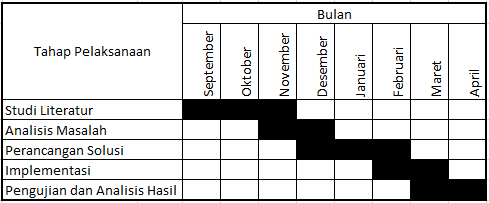
\includegraphics[width=0.8\textwidth]{resources/chapter-1-gantt-chart.png}
    \caption{Rencana jadwal pelaksanaan tugas akhir}
\end{figure}